\documentclass[conference]{IEEEtran}
\IEEEoverridecommandlockouts
% The preceding line is only needed to identify funding in the first footnote. If that is unneeded, please comment it out.
\usepackage{cite}
\usepackage{amsmath,amssymb,amsfonts}
\usepackage{algorithmic}
\usepackage{graphicx}
\usepackage{textcomp}
\usepackage{xcolor}
\usepackage{hyperref}

\newcommand{\gr}[1]{\textcolor{green}{#1}}

\def\BibTeX{{\rm B\kern-.05em{\sc i\kern-.025em b}\kern-.08em
    T\kern-.1667em\lower.7ex\hbox{E}\kern-.125emX}}
\begin{document}

\title{Mamba vs SOTA for Vision Tasks\\
    \thanks{$\dagger$ Equal contributions}
}

\author{\IEEEauthorblockN{Clay Crews$^{\dagger}$}
    \IEEEauthorblockA{\textit{Department of Computer Science} \\
        \textit{University of South Carolina}\\
        Columbia, SC, United States \\
        jccrews@email.sc.edu}
    \and
    \IEEEauthorblockN{Lexington Whalen$^{\dagger}$}
    \IEEEauthorblockA{\textit{Department of Computer Science} \\
        \textit{University of South Carolina}\\
        Columbia, SC, United States\\
        LAWHALEN@email.sc.edu}
}

\maketitle

\begin{abstract}
    Abstract
    This paper explores the performance of the Mamba architecture, a variant of Structured State Space Sequence Models (SSMs), in comparison to state-of-the-art models such as Transformers, U-Net, and ResNet for vision tasks. We focus on image segmentation and classification, with the goal of maintaining high accuracy while keeping parameter counts low. Developing compact models with fewer parameters is crucial for the future of AI, not only to reduce energy consumption but also to enable deployment on resource-constrained edge devices.
    By leveraging the selective state spaces in Mamba blocks, we aim to achieve efficient and effective segmentation and classification performance while maintaining the linear scalability of SSMs. We implement Mamba-based architectures and compare their results to popular models like U-Net, ResNet, and Transformer-based approaches on standard vision benchmarks.
    In addition to accuracy, we place a strong emphasis on model size, targeting compact architectures suitable for resource-constrained environments. Through careful design choices and optimizations, we strive to develop Mamba-based models that achieve competitive accuracy with significantly fewer parameters compared to existing state-of-the-art models.
    This work highlights the potential of Mamba and SSMs for efficient vision tasks, contributing to the development of compact yet accurate models in image segmentation and classification. We open-source our code to facilitate further research and exploration of these architectures: \href{https://github.com/lxaw/mamba-vs-else-vision}{https://github.com/lxaw/mamba-vs-else-vision}
\end{abstract}

\begin{IEEEkeywords}
    Mamba, TinyML, Image Segmentation, Image Classification
\end{IEEEkeywords}

\section{Introduction}
The rapid advancement of deep learning has led to remarkable achievements in various domains, including computer vision, natural language processing, and speech recognition. However, this progress has been accompanied by a significant increase in the size and complexity of neural network models. State-of-the-art models often have hundreds of millions or even billions of parameters, making them computationally expensive and challenging to deploy on resource-constrained devices \cite{brown2020language, dosovitskiy2021image}. This trend poses concerns regarding energy consumption and the feasibility of deploying these models on edge devices, which have limited memory and processing power.

The growth of edge devices and the emerging field of TinyML have highlighted the need for more efficient and compact models \cite{warden2019tinyml}. Edge devices, such as smartphones, wearables, and IoT sensors, have become increasingly prevalent in our daily lives. These devices often require real-time processing and decision-making capabilities, but their limited resources make it challenging to run large, complex models. TinyML aims to address this challenge by developing machine learning techniques that can operate efficiently on resource-constrained devices, enabling a wide range of intelligent applications at the edge \cite{banbury2021benchmarking}.

Many state-of-the-art models for vision tasks, such as image classification and segmentation, rely on architectures like Transformers \cite{dosovitskiy2021image}, U-Net \cite{ronneberger2015unet}, and ResNet \cite{he2016deep}. While these models have achieved impressive performance, they often come with a high parameter count. Transformers, in particular, have gained significant attention due to their ability to capture long-range dependencies and achieve superior results in various tasks \cite{vaswani2017attention}. However, the self-attention mechanism in Transformers scales quadratically with the input sequence length, making them computationally expensive and difficult to apply to long sequences or high-resolution images \cite{choromanski2020rethinking}.

To address the challenges of large parameter models and enable efficient deployment on edge devices, there is a growing interest in developing more compact and computationally efficient architectures. One promising approach is the Mamba architecture, which is based on Structured State Space Sequence Models (SSMs) \cite{gu2022efficiently}. Mamba combines the modeling power of Transformers with the linear scalability of SSMs, allowing it to efficiently process long sequences while maintaining high performance \cite{gu2023mamba}. By leveraging selective state spaces, Mamba can achieve competitive results with significantly fewer parameters compared to Transformers and other large models.

In this paper, we explore the application of Mamba for vision tasks, specifically image segmentation and classification. We aim to demonstrate that Mamba-based models can achieve high accuracy while keeping parameter counts low, making them suitable for deployment on edge devices and contributing to the development of more sustainable and efficient AI solutions. We compare the performance of Mamba against state-of-the-art models and discuss the potential of this approach for enabling intelligent applications on resource-constrained devices.
\section{Current Vision Task SOTA}
Over the past decade, deep learning has revolutionized the field of computer vision, with various architectures achieving state-of-the-art (SOTA) performance on tasks such as image classification and segmentation. Convolutional Neural Networks (CNNs) have been at the forefront of this revolution, with architectures like AlexNet \cite{krizhevsky2012imagenet}, VGGNet \cite{simonyan2014very}, and Inception \cite{szegedy2015going} pushing the boundaries of classification accuracy on large-scale datasets like ImageNet.
One of the most significant advancements in CNNs came with the introduction of ResNet \cite{he2016deep}, which addressed the problem of vanishing gradients in deep networks by introducing residual connections. ResNets allowed for the training of much deeper networks, leading to improved performance on various vision tasks. The success of ResNet sparked a wave of research into more efficient and effective CNN architectures, such as MobileNet \cite{howard2017mobilenets}, EfficientNet \cite{tan2019efficientnet}, and RegNet \cite{radosavovic2020designing}.
While CNNs have been highly successful in vision tasks, they struggle to capture long-range dependencies and global context, which are crucial for understanding complex scenes and objects. To address this limitation, the Vision Transformer (ViT) \cite{dosovitskiy2021image} was introduced, adapting the self-attention mechanism from natural language processing to vision tasks. ViT treats an image as a sequence of patches and applies multi-head self-attention to learn global relationships between these patches. ViT has achieved impressive results on image classification tasks, often outperforming CNNs while requiring less inductive bias.
Building upon the success of ViT, several transformer-based architectures have been proposed for other vision tasks, such as image segmentation. SegFormer \cite{xie2021segformer} is a transformer-based model for semantic segmentation that employs a hierarchical structure and a novel attention mechanism called Efficient Self-Attention (ESA). ESA reduces the computational complexity of self-attention by performing attention operations in a local window and aggregating global information through a depth-wise convolution. This allows SegFormer to efficiently process high-resolution images while capturing both local and global context.
Despite the impressive performance of these SOTA models, they often come with a high computational cost and large number of parameters. The self-attention mechanism in transformers scales quadratically with the input sequence length, making them challenging to apply to long sequences or high-resolution images \cite{choromanski2020rethinking}. CNNs, while more efficient than transformers, still require a significant number of parameters to achieve SOTA performance, especially for complex tasks like segmentation.
The high parameter counts and scaling issues of these models pose challenges for deployment on resource-constrained devices and raise concerns about energy consumption. As the demand for efficient and sustainable AI solutions grows, there is a pressing need for more compact and computationally efficient architectures that can maintain high accuracy while reducing the parameter footprint. This has led to increased interest in techniques like model compression, quantization, and the development of novel architectures that can achieve SOTA performance with fewer parameters \cite{cheng2017survey, hinton2015distilling}.

\section{State Space Models (SSMs)}
State Space Models (SSMs) are a powerful mathematical framework for modeling and processing temporal signals. They map an input signal $u(t)$ to an output signal $y(t)$ via a latent state $x(t)$. The latent state evolves according to a linear differential equation involving the input signal and a set of matrices $(A, B, C, D)$ that define the SSM's behavior \cite{gu2022efficiently}.
When the SSM matrices are constant over time, the system is called a Linear Time-Invariant (LTI) SSM, and it can be equivalently expressed as a convolution between the input signal and the SSM's impulse response function $K(t)$. This convolutional form makes LTI SSMs particularly efficient to compute, which is crucial for their application in modern deep learning models like S4 \cite{gu2022efficiently}.
A key concept in the SSM literature is the SSM basis, which is a set of functions defined by the matrix exponential $e^{tA}B$. The output of the SSM is a linear combination of these basis functions, weighted by the coefficients in matrix $C$. The choice of the SSM basis functions determines the properties and capabilities of the SSM \cite{gu2022efficiently}.
The HiPPO framework proposed a mathematical technique for deriving SSMs with orthogonal basis functions, such that the latent state $x(t)$ maintains a compressed representation of the entire input history. By carefully designing the SSM matrices, HiPPO derived SSMs whose basis functions could reconstruct the input signal history from the latent state, making them powerful tools for modeling long-range dependencies in sequence data \cite{gu2020hippo}.
The Mamba model built upon the foundations laid by HiPPO, extending SSMs with a gating mechanism to enable more general sequence modeling tasks beyond signal reconstruction and memorization \cite{gu2023mamba}. The success of models like S4 and Mamba have demonstrated the potential of SSMs as a fundamental building block for efficient and expressive sequence models.

\section{Mamba}
Mamba \cite{gu2023mamba} is a recently proposed architecture that combines the modeling power of Transformers with the linear scaling efficiency of state space models (SSMs). The key idea is to augment SSMs with a selection mechanism that allows the model parameters to vary based on the input, enabling it to perform content-aware reasoning.
Standard SSMs map an input sequence $x(t)$ to an output $y(t)$ via a latent state $h(t)$ using a linear time-invariant system:
\begin{align*}
h'(t) & = \mathbf{A}h(t) + \mathbf{B}x(t) \\
y(t)  & = \mathbf{C}h(t) + \mathbf{D}x(t)
\end{align*}
where the parameter matrices $\mathbf{A}$, $\mathbf{B}$, $\mathbf{C}$, $\mathbf{D}$ are fixed. In the original paper, the $\mathbf{D}$ matrix is considered only as a skip connection, and thus as it does not directly play a role in the differential equation, was ignored. This allows SSMs to be computed efficiently as a convolution. However, the time-invariance means the model cannot change its behavior for specific inputs, making it difficult to solve tasks requiring selective focus, such as selective copying or induction heads \cite{gu2023mamba}.
Mamba introduces a selection mechanism where the SSM parameters $\mathbf{B}$, $\mathbf{C}$, $\Delta$ (the state step size) vary for each input token $x_t$. This allows the model to selectively propagate or forget information based on the current token. The selective SSM is computed using a parallel scan operation to maintain linear complexity.
The Mamba block interleaves the selective SSM with linear projections, convolutions, and activations:
\begin{enumerate}
\item Linear projection to expand the embedding dimension
\item Convolution to mix information between dimensions
\item Selective SSM via parallel scan to efficiently propagate information
\item Linear projection to get back to the target embedding size
\end{enumerate}
These blocks are stacked to form the Mamba architecture. Compared to Transformers, Mamba can achieve comparable modeling performance while scaling linearly in sequence length rather than quadratically \cite{gu2023mamba}. Overall, the selective SSM leverages the strengths of RNNs, CNNs and Transformers - it maintains an unbounded context window like RNNs, can be parallelized like CNNs, and achieves content-aware reasoning like Transformers, while being more efficient than all three. This makes Mamba a promising foundation model for processing long sequences across various domains.

\section{Application: Image Segmentation}
Here we investigate Mamba-based architectures with regards to the task of image segmentation.

\section{Input Data}\label{sec2}
We shall be using a Brain MRI segmentation dataset found in \cite{dataset}. This dataset has been used in several papers regarding classification of the shape and severity of tumors, and provides an adequate dataset for research purposes in the field of medical image analysis, particularly in the area of brain MRI segmentation. Researchers have utilized this dataset in various studies focusing on the classification of tumor shapes and the assessment of tumor severity. With its comprehensive collection of brain MRI scans, along with corresponding segmentation masks, the dataset offers valuable resources for developing and evaluating algorithms aimed at automating tumor detection and analysis.

The dataset contains brain MRI images along with their segmentation masks for 110 patients. There were a total of 3143 train images, 393 validation images, and 393 test images. The distribution of the tumor and non-tumor images is shown in Figure \ref{fig:datastats}.


\section{Output Data}\label{sec3}
The output of this model shall be segmentation masks for new, never before seen images.
\begin{figure}[!t]
    \centering
    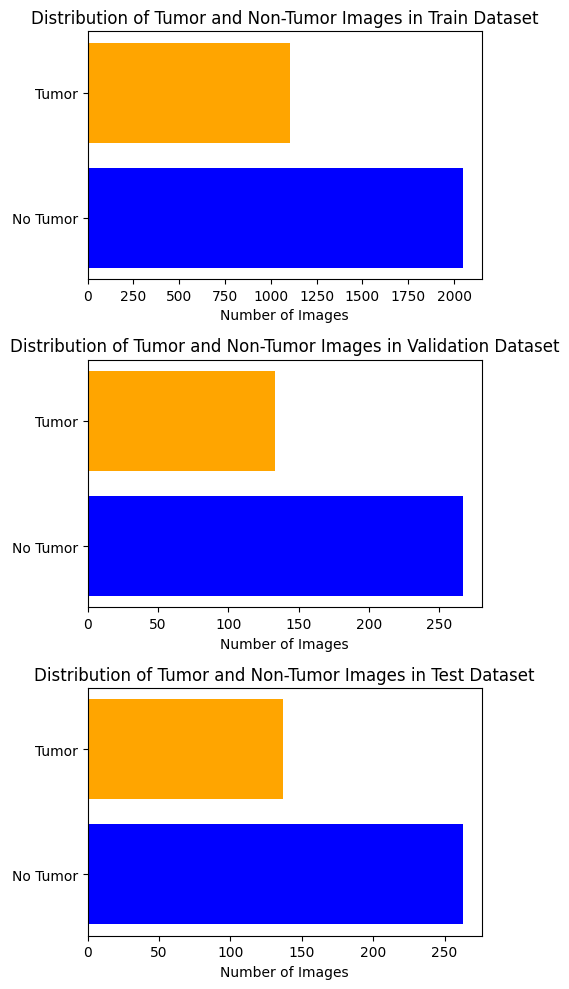
\includegraphics[width=\columnwidth]{imgs/data_stats.png}
    \caption{Distributions of tumor and non-tumor images in the train, validation, and test datasets.}
    \label{fig:datastats}
\end{figure}

\section{Compared Models}
Prior to an analysis of how the Pyramidal U-Mamba compares, we shall explain what models we chose for comparison and why.

For this our analysis, we compare four models against our own developed ones. The models are U-Net\cite{ronneberger2015unet}, ResNet18 \cite{DBLP:journals/corr/HeZRS15}, ResNet50, U-Mamba\cite{U-Mamba}, and SegViT\cite{dosovitskiy2021image}. Below we explain our choices.
\subsection{U-Net}
The core idea behind U-Net is to complement a traditional contracting network with successive layers that replace pooling operations with upsampling operators. These upsampling layers aim to increase the resolution of the output. Subsequent convolutional layers can then learn to assemble a precise output based on this high-resolution information \cite{ronneberger2015unet}.
A key modification in the U-Net architecture is the inclusion of a large number of feature channels in the upsampling part. This allows the network to effectively propagate contextual information to higher resolution layers. As a result, the expansive path of the network becomes more or less symmetric to the contracting part, leading to a distinctive U-shaped architecture. To predict pixels at the border regions of the image, the missing context is extrapolated by mirroring the input image. This tiling strategy is crucial for applying the network to large images, as it circumvents resolution limitations imposed by GPU memory constraints \cite{ronneberger2015unet}. Due to its encoder-decoder architecture, skip connections, multi-scale feature extraction, and its efficiency, U-Net has been used in many denoising and diffusion models. For instance, DDPMs (Denoising Diffusion Probabilistic Models) use an architecture similar to U-Net for denoising and sample generation \cite{DBLP:journals/corr/abs-2006-11239} while the popular Stable Diffusion architecture uses a U-Net based architecture for the diffusion process \cite{rombach2021highresolution}. We have chosen to compare our novel segmentation architecture against the U-Net architecture due to its well-established reputation and widespread adoption in the field of medical image segmentation.

\subsection{ResNet}
We have also selected ResNet18 and ResNet50 as additional benchmarks. These architectures, introduced by He et al. in their seminal work "Deep Residual Learning for Image Recognition" \cite{DBLP:journals/corr/HeZRS15}, have revolutionized the field of deep learning by addressing the problem of vanishing gradients in deep neural networks. The key innovation in ResNets is the introduction of residual connections, which allow the network to learn residual functions with reference to the input layer, thereby facilitating the training of much deeper networks. ResNet18 and ResNet50, with 18 and 50 layers respectively, have been widely adopted in various computer vision tasks, including image classification, object detection, and segmentation. These models have demonstrated exceptional performance and generalization ability across diverse datasets. By comparing our proposed architecture against ResNet18 and ResNet50, we aim to assess its effectiveness in relation to these well-established and highly influential architectures. This comparison will provide valuable insights into the capabilities of our model and its potential to advance the state-of-the-art in image segmentation tasks.
\subsection{U-Mamba}
As our model takes much inspiration from the recently developed U-Mamba design \cite{U-Mamba}, we also choose to incorporate it in our comparison. U-Mamba addresses these limitations by introducing a novel hybrid CNN-SSM block that leverages the strengths of both architectures. The convolutional layers in the block are responsible for local feature extraction, while the State Space Sequence Models (SSMs) \cite{gu2022efficiently}, a new family of deep sequence models, are known for their strong capability in handling long sequences and capturing long-range dependencies. By integrating these two components, U-Mamba achieves a balance between local and global information processing, enabling it to effectively handle long-range dependencies in biomedical image segmentation tasks. Moreover, U-Mamba incorporates a self-configuring mechanism that allows it to automatically adapt to various datasets without manual intervention, enhancing its versatility and usability.
\subsection{SegFormer}
SegFormer \cite{xie2021segformer} is a transformer-based semantic segmentation model that employs a hierarchical structure and a novel attention mechanism called Efficient Self-Attention (ESA). The SegFormer architecture consists of a transformer encoder for capturing long-range dependencies and a lightweight All-MLP decoder for generating high-resolution segmentation masks. The ESA module reduces the computational complexity of self-attention by performing attention operations in a local window and aggregating global information through a depth-wise convolution. This allows SegFormer to efficiently process high-resolution images while capturing both local and global context. Moreover, SegFormer introduces a position-sensitive embedding scheme that encodes both spatial and channel-wise information, enhancing the model's ability to capture fine-grained details. By comparing U-Mamba against SegFormer, we aim to evaluate the effectiveness of our hybrid CNN-SSM approach in relation to the transformer-based segmentation mechanism employed by SegFormer. This comparison will provide insights into the strengths and weaknesses of both architectures and their ability to handle complex biomedical image segmentation tasks. Furthermore, it will help us understand the potential of transformer-based approaches and hybrid approaches in advancing the state-of-the-art in biomedical image segmentation.

\subsection{UltraLight VM-UNet}
The UltraLight VM-UNet \cite{ultralightvmunet} is a lightweight neural network architecture designed for skin lesion segmentation tasks. It is built upon the Vision Mamba module, which is a state-space model (SSM) that can efficiently handle long-range dependencies in sequences, making it well-suited for image segmentation tasks.

The key innovation of the UltraLight VM-UNet is the proposed Parallel Vision Mamba Layer (PVM Layer), which processes deep features in parallel using multiple Vision Mamba blocks. Specifically, the input feature map is split into multiple sub-feature maps, each processed by a separate Vision Mamba block with a reduced channel count. This parallel processing approach allows the UltraLight VM-UNet to maintain high segmentation performance while significantly reducing the number of parameters and computational complexity.

The UltraLight VM-UNet is reported to have only 0.049 million parameters and a computational cost of 0.060 GFLOPs, which is significantly lower than traditional convolutional neural networks and transformers used for image segmentation tasks. Despite its lightweight nature, the authors demonstrate that the UltraLight VM-UNet achieves competitive performance on three publicly available skin lesion segmentation datasets, outperforming several state-of-the-art lightweight models.

The success of the UltraLight VM-UNet can be attributed to the authors' in-depth analysis of the key factors influencing the parameters of the Vision Mamba module. By identifying the number of input channels as a critical factor affecting the parameter count, they were able to design the PVM Layer to process features in parallel while keeping the overall channel count constant, leading to a significant reduction in parameters without compromising performance.

\section{Our Models}

Inspired by \cite{U-Mamba} and \cite{ultralightvmunet}, we sought to implement both models on a different problem: tumor segmentation.

Our goal was to 1) maintain dice scores comparable to state-of-the-art (SOTA) methods such as those listed above, while 2) being smaller than those above.

We now go into what we did for each of our models.


\subsection{UMambaBot\_PPBot}

This model incorporates pyramidal pooling, which is a strategy used in convolutional neural networks (CNNs) to capture context and incorporate multi-scale information \cite{zhao2017pyramid}. Pyramidal pooling involves parallel pooling operations at different scales, followed by concatenation of the resulting feature maps. This approach has been shown to improve the performance of CNNs in various computer vision tasks, including segmentation, by enabling the model to capture both local and global context.

In our UMambaBot\_PP model, we integrated pyramidal pooling into the U-Mamba architecture, aiming to leverage the strengths of both the Mamba module and multi-scale feature extraction.

% Unsure why this comment line is giving me troubles !!

\subsection{UL-VM-UNet\_v1}
For ULMUNet\_v1, the initial channel list was modified from [8, 16, 24, 32, 48, 64] to [16, 32, 64, 128, 256], increasing the number of channels at each step of the encoder and decoder. Additionally, the depth of the U-Net was reduced by one layer to keep the parameter count low while increasing the number of parameters in each step. The intention was to improve performance by increasing the capacity of the model while maintaining a reasonable parameter count.

\subsection{UL-VM-UNet\_v2}
In ULMUNet\_v2, the number of parallel branches in the Parallel Vision Mamba (PVM) block was increased from 4 to 8. This modification directly decreases the parameter count, further proving the idea proposed in the UltraLight VM-UNet paper \cite{ultralightvmunet} that processing features in parallel with reduced channel counts can significantly reduce parameters while maintaining performance.

\subsection{UL-VM-UNet\_v3}
ULMUNet\_v3 combines the modifications from ULMUNet\_v1 and ULMUNet\_v2. It increases the number of parallel branches in the PVM block to 8 and modifies the channel list to [16, 32, 64, 128, 256]. Additionally, the depth of the U-Net was reduced to 5 layers. This approach aims to balance the trade-off between model capacity and parameter efficiency.

\subsection{UL-VM-UNet\_v4}
\gr{Pyramidal pooling was used in each of the PVM blocks in the encoder and decoder networks. If we want to do similar to UMambaBot\_PP we can do it just in the bottleneck. Let me know if we want this can I can do it fast.}
This model incorporates pyramidal pooling, similar to UMambaBot\_PP, but within the UltraLight VM-UNet architecture. The goal was to leverage the benefits of multi-scale feature extraction while maintaining the parameter efficiency of the UltraLight VM-UNet.

\subsection{UL-VM-UNet\_v5}
\gr{What is UL-PP? v5 is v4 with no PP. If any, v4 is UL-PP.}
The UL-PP (Ultra Light Pyramidal Pooling) model trained and performed well with 1.1M parameters. Incorporating pyramidal pooling on the UL network scored slightly worse than without pyramidal pooling but required approximately 400,000 more parameters.


\section{Results}
We now compare our models against ResNet18, ResNet50, standard U-Mamba bottleneck, UNet, and UltraLight VM-UNet. We train for 100 epochs on all models, and use dice-loss with Adam optimizer. We train on roughly 3000 images, and validate on roughly 400. we then test on roughly 400. We show the stats of our data in Figure \ref{fig:datastats}.
The results are shown in Figures \ref{fig:balls} and \ref{fig:segs}.

\begin{table}[ht]
    \centering
    \begin{tabular}{|l|c|c|}
        \hline
        \textbf{Model Name} & \textbf{Parameter Count (Millions)} & \textbf{Dice Score} \\
        \hline
        UMambaBot\_PP & 10.0 & 0.8867 \\
        UMambaBot & 9.8 & 0.8799 \\
        ResNet18 & 13.9 & 0.8648 \\
        ResNet50 & 42.9 & 0.8672 \\
        SegFormer & 17.8 & 0.8454 \\
        UNet & 7.8 & 0.8929 \\
        UL-VM-UNet & 0.049 & 0.79955 \\
        UL-VM-UNet\_v1 & 0.20 & 0.8409 \\
        UL-VM-UNet\_v2 & 0.042 & 0.8243 \\
        UL-VM-UNet\_v3 & 0.176 & 0.8109 \\
        UL-VM-UNet\_v4 & 1.1 & 0.8548 \\
        UL-VM-UNet\_v5 & 0.7 & 0.8633 \\
        \hline
    \end{tabular}
    \caption{Comparison of different segmentation models.}
    \label{tab:model_comparison}
\end{table}

\begin{figure}[!t]
    \centering
    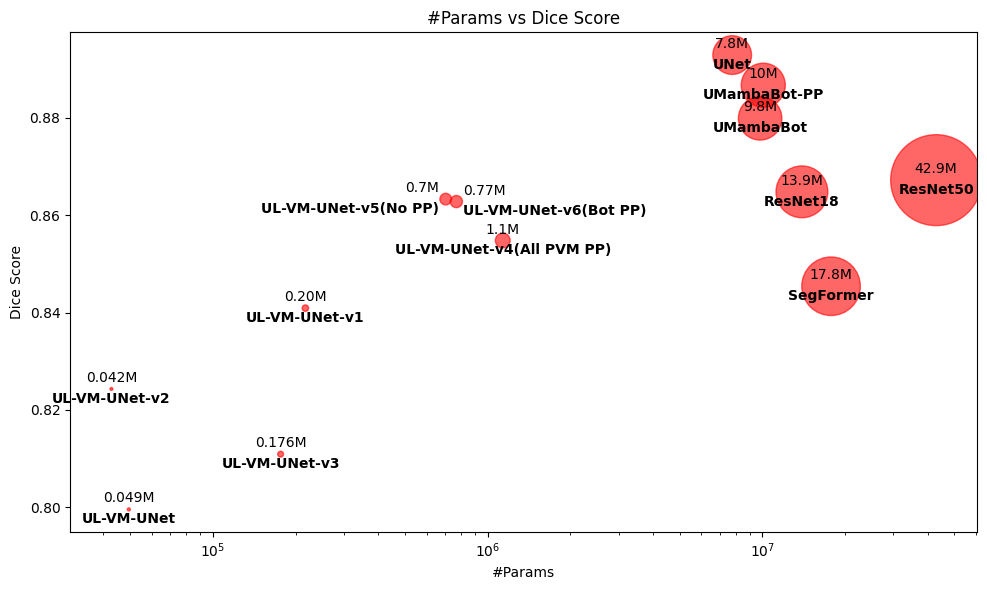
\includegraphics[width=\columnwidth]{imgs/balls.png}
    \caption{A scatter plot of Dice Score vs model parameter count, where "M" means "millions. The points are scaled to help represent size.}
    \label{fig:balls}
\end{figure}

\begin{figure}[!t]
    \centering
    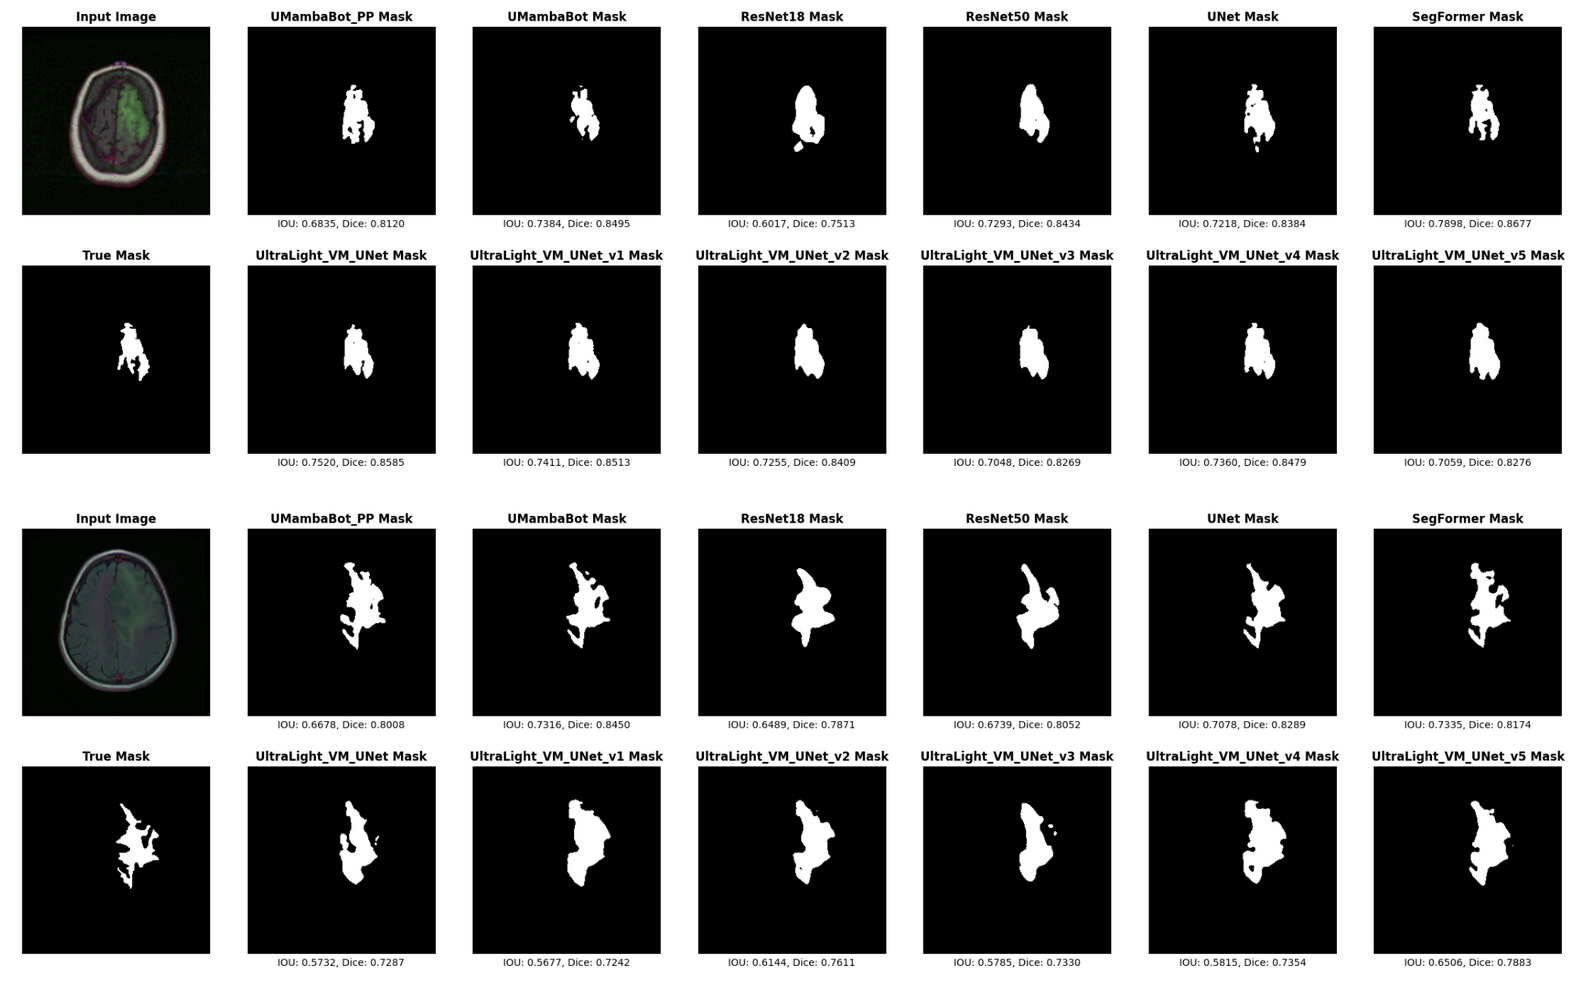
\includegraphics[width=\columnwidth]{imgs/masks.png}
    \caption{Example segmentations.}
    \label{fig:segs}
\end{figure}

\section{Application: Image Classsification}

\section{Conclusion}


\begin{thebibliography}{00}
\bibitem{brown2020language} T. B. Brown et al., "Language Models are Few-Shot Learners," arXiv:2005.14165 [cs.CL], 2020.
\bibitem{dosovitskiy2021image} A. Dosovitskiy et al., "An Image is Worth 16x16 Words: Transformers for Image Recognition at Scale," arXiv:2010.11929 [cs.CV], 2021.
\bibitem{warden2019tinyml} P. Warden and D. Situnayake, "TinyML: Machine Learning with TensorFlow Lite on Arduino and Ultra-Low-Power Microcontrollers," O'Reilly Media, Inc., 2019.
\bibitem{banbury2021benchmarking} C. R. Banbury et al., "MLPerf Tiny Benchmark," arXiv:2106.07597 [cs.LG], 2021.
\bibitem{ronneberger2015unet} O. Ronneberger, P. Fischer, and T. Brox, "U-Net: Convolutional Networks for Biomedical Image Segmentation," arXiv:1505.04597 [cs.CV], 2015.
\bibitem{he2016deep} K. He, X. Zhang, S. Ren, and J. Sun, "Deep Residual Learning for Image Recognition," arXiv:1512.03385 [cs.CV], 2016.
\bibitem{vaswani2017attention} A. Vaswani et al., "Attention Is All You Need," arXiv:1706.03762 [cs.CL], 2017.
\bibitem{choromanski2020rethinking} K. Choromanski et al., "Rethinking Attention with Performers," arXiv:2009.14794 [cs.LG], 2020.
\bibitem{gu2022efficiently} A. Gu, K. Goel, and C. Ré, "Efficiently Modeling Long Sequences with Structured State Spaces," arXiv:2111.00396 [cs.LG], 2022.
\bibitem{gu2023mamba} A. Gu and T. Dao, "Mamba: Linear-Time Sequence Modeling with Selective State Spaces," arXiv:2312.00752 [cs.LG], 2023.
\bibitem{krizhevsky2012imagenet} - ImageNet Classification with Deep Convolutional Neural Networks
\bibitem{simonyan2014very} - Very Deep Convolutional Networks for Large-Scale Image Recognition
\bibitem{szegedy2015going} - Going Deeper with Convolutions
\bibitem{he2016deep} - Deep Residual Learning for Image Recognition
\bibitem{howard2017mobilenets} - MobileNets: Efficient Convolutional Neural Networks for Mobile Vision Applications
\bibitem{tan2019efficientnet} - EfficientNet: Rethinking Model Scaling for Convolutional Neural Networks
\bibitem{radosavovic2020designing} - Designing Network Design Spaces
\bibitem{dosovitskiy2021image} - An Image is Worth 16x16 Words: Transformers for Image Recognition at Scale
\bibitem{xie2021segformer} - SegFormer: Simple and Efficient Design for Semantic Segmentation with Transformers
\bibitem{choromanski2020rethinking} - Rethinking Attention with Performers
\bibitem{cheng2017survey} - A Survey of Model Compression and Acceleration for Deep Neural Networks
\bibitem{hinton2015distilling} - Distilling the Knowledge in a Neural Network
\bibitem{gu2022efficiently} A. Gu, K. Goel, and C. Ré, "Efficiently Modeling Long Sequences with Structured State Spaces," arXiv preprint arXiv:2111.00396, 2022.
\bibitem{gu2020hippo} A. Gu, T. Dao, S. Ermon, A. Rudra, and C. Ré, "HiPPO: Recurrent Memory with Optimal Polynomial Projections," Advances in Neural Information Processing Systems, vol. 33, pp. 1474-1487, 2020.
\bibitem{gu2023mamba} A. Gu and T. Dao, "Mamba: Linear-Time Sequence Modeling with State Spaces," arXiv preprint arXiv:2302.01327, 2023.
\bibitem{ronneberger2015unet} O. Ronneberger, P. Fischer, and T. Brox, "U-Net: Convolutional Networks for Biomedical Image Segmentation," arXiv:1505.04597 [cs.CV], 2015.

\bibitem{vaswani2023attention} A. Vaswani et al., "Attention Is All You Need," arXiv:1706.03762 [cs.CL], 2023.

\bibitem{gu2022efficiently} A. Gu, K. Goel, and C. Ré, "Efficiently Modeling Long Sequences with Structured State Spaces," arXiv:2111.00396 [cs.LG], 2022.

\bibitem{gu2023mamba} A. Gu and T. Dao, "Mamba: Linear-Time Sequence Modeling with Selective State Spaces," arXiv:2312.00752 [cs.LG], 2023.

\bibitem{bakas2019identifying} S. Bakas et al., "Identifying the Best Machine Learning Algorithms for Brain Tumor Segmentation, Progression Assessment, and Overall Survival Prediction in the BRATS Challenge," arXiv:1811.02629 [cs.CV], 2019.

\bibitem{U-Mamba} J. Ma, F. Li, and B. Wang, "U-Mamba: Enhancing Long-range Dependency for Biomedical Image Segmentation," arXiv:2401.04722 [cs.CV], 2024.

\bibitem{rombach2021highresolution} R. Rombach, A. Blattmann, D. Lorenz, P. Esser, and B. Ommer, "High-Resolution Image Synthesis with Latent Diffusion Models," arXiv:2112.10752 [cs.CV], 2021.

\bibitem{DBLP:journals/corr/abs-2006-11239} J. Ho, A. Jain, and P. Abbeel, "Denoising Diffusion Probabilistic Models," CoRR, vol. abs/2006.11239, 2020. [Online]. Available: https://arxiv.org/abs/2006.11239

\bibitem{DBLP:journals/corr/HeZRS15} K. He, X. Zhang, S. Ren, and J. Sun, "Deep Residual Learning for Image Recognition," CoRR, vol. abs/1512.03385, 2015. [Online]. Available: http://arxiv.org/abs/1512.03385

\bibitem{zhang2022segvit} B. Zhang et al., "SegViT: Semantic Segmentation with Plain Vision Transformers," arXiv:2210.05844 [cs.CV], 2022.

\bibitem{dosovitskiy2021image} A. Dosovitskiy et al., "An Image is Worth 16x16 Words: Transformers for Image Recognition at Scale," arXiv:2010.11929 [cs.CV], 2021.
\bibitem{ultralightvmunet} R. Wu, Y. Liu, P. Liang, and Q. Chang, “UltraLight VM-UNet: Parallel Vision Mamba Significantly Reduces Parameters for Skin Lesion Segmentation.” Accessed: Apr. 20, 2024. [Online]. Available: https://arxiv.org/pdf/2403.20035.pdf
\bibitem{zhao2017pyramid}
H. Zhao, J. Shi, X. Qi, X. Wang and J. Jia, "Pyramid Scene Parsing Network," 2017 IEEE Conference on Computer Vision and Pattern Recognition (CVPR), 2017, pp. 6230-6239, doi: 10.1109/CVPR.2017.660.
\bibitem{dataset} “Brain MRI segmentation,” www.kaggle.com. https://www.kaggle.com/datasets/mateuszbuda/lgg-mri-segmentation
\bibitem{xie2021segformer} E. Xie, W. Wang, Z. Yu, A. Anandkumar, J. Alvarez, and P. Luo, “SegFormer: Simple and Efficient Design for Semantic Segmentation with Transformers.” Available: https://arxiv.org/pdf/2105.15203.pdf
\end{thebibliography}

\end{document}
